\newpage
\section{Auswertung}
    \subsection{Ausmessung des Magnetfeldes}
        \begin{figure}[h]
            \centering
            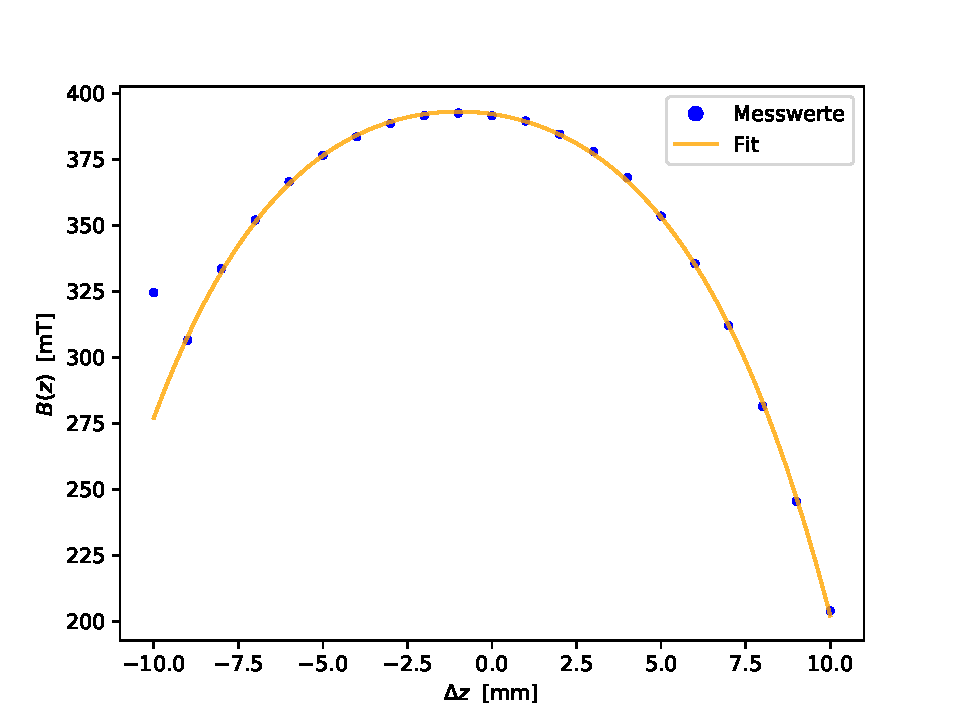
\includegraphics[width = 0.7\textwidth]{plots/Magnetfeld.pdf}
            \caption{Die Magnetfeldstärke $B(z)$ ist gegen den Abstand zum Ort der Proben aufgetragen.}
            \label{fig:Magnetfeld}
        \end{figure}

        \FloatBarrier
    
        Um die maximale Feldstärke $B_{\text{max}}$ zu bestimmen wird ein Fit der Funktion
        \begin{equation*}
            f(x) = ax^4 + bx^3 + cx^2 + dx + e
        \end{equation*}
        durch die Messwerte gelegt. Diese ergibt sich daraus zu $B_{\text{max}} \approx 0,393 \,$mT und wird im Nachfolgenden in den Berechnungen zur effektiven Masse benutzt.

    \subsection{Darstellung der Messwerte}
        Wie schon beschrieben wurden zwei Messreihen pro Probe aufgenommen, jeweils für eine Richtung des Magnetfeldes. Für jede Probe wird die Faraday-Rotation nach \autoref{eqn:zweiwinkel} bestimmt.
        
        Da alle drei Proben verschiedene Dicken haben muss der Winkel der Faraday-Rotation zuerst auf die jeweilige Dicke $L$ der Probe normiert werden, bevor die Winkel miteinander verglichen und verrechnet werden können. Dies führt dann zu der folgenden Formel für die normierten Winkel:
        \begin{equation*}
            \theta_{\text{norm}} = \frac{\theta_1 - \theta_2}{2 L}
        \end{equation*}
        
        \begin{figure}[h]
            \centering
            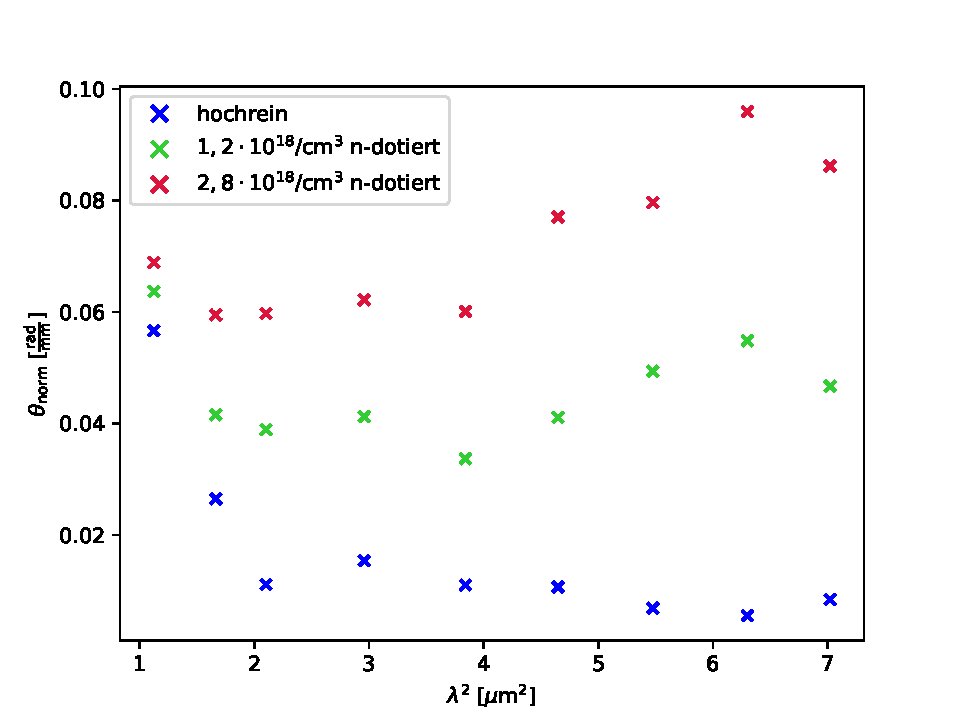
\includegraphics[width = 0.75\textwidth]{plots/Winkel_normiert.pdf}
            \caption{Die normierten Winkel der Faraday-Rotation für jede der drei Proben sind gegen die quadrierte betrachtete Wellenlänge aufgetragen.}
            \label{fig:Winkel_normiert}
        \end{figure}

        \FloatBarrier

    \subsection{Bestimmung der effektiven Masse}
        Um die effektive Masse freier Elektronen zu bestimmen werden n-dotierte Proben benutzte, da diese freie Elektronen mitbringen welche die Differenz zwischen den normierten Winkeln der hochreinen und den zwei n-dotierten Proben gebildet $\Delta \theta_{\text{norm}} = \theta_{\text{norm,dot}} - \theta_{\text{norm,rein}}$ verursachen.

        Nach \eqref{eqn:faraday} sollte der Winkel der Faraday-Rotation proportional zur quadrierten Wellenlänge sein.
        Deshalb wird durch die Messwerte in \autoref{fig:Faraday_1} und \autoref{fig:Faraday_2} jeweils ein linearer Fit gelegt
        \begin{equation*}
            f(x) = a \cdot x
        \end{equation*}
        wobei sich die für die beiden dotierten Proben die folgenden Steigungen ergeben:
        \begin{align*}
            m_1 = (0,00701 \pm 0,00054) \, \frac{\text{rad}}{\mu \text{m}^2 \cdot \text{mm}} \\[7pt]
            m_2 = (0,01345 \pm 0,00082) \, \frac{\text{rad}}{\mu \text{m}^2 \cdot \text{mm}}
        \end{align*}
    
        \begin{figure}[h]
            \centering
            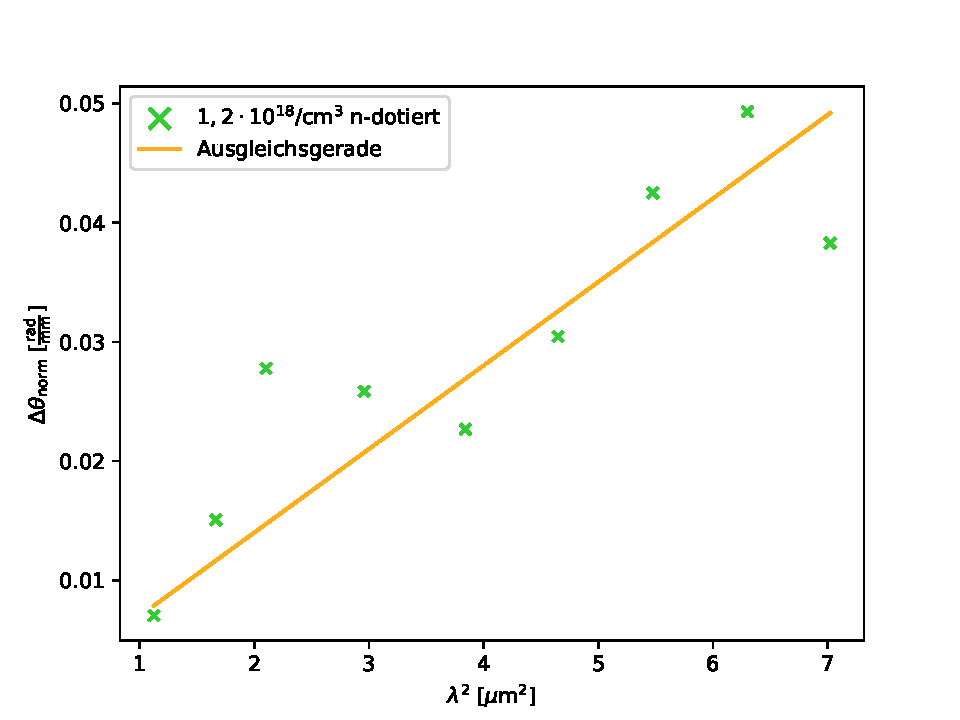
\includegraphics[width = 0.8\textwidth]{plots/Faraday_1.pdf}
            \caption{Die Differenz der Faraday-Rotation zwischen der hochreinen und ersten dotierten Probe wird gegen die quadrierte Wellenlängeaufgetragen.}
            \label{fig:Faraday_1}
        \end{figure}

        \FloatBarrier

        \begin{figure}[h]
            \centering
            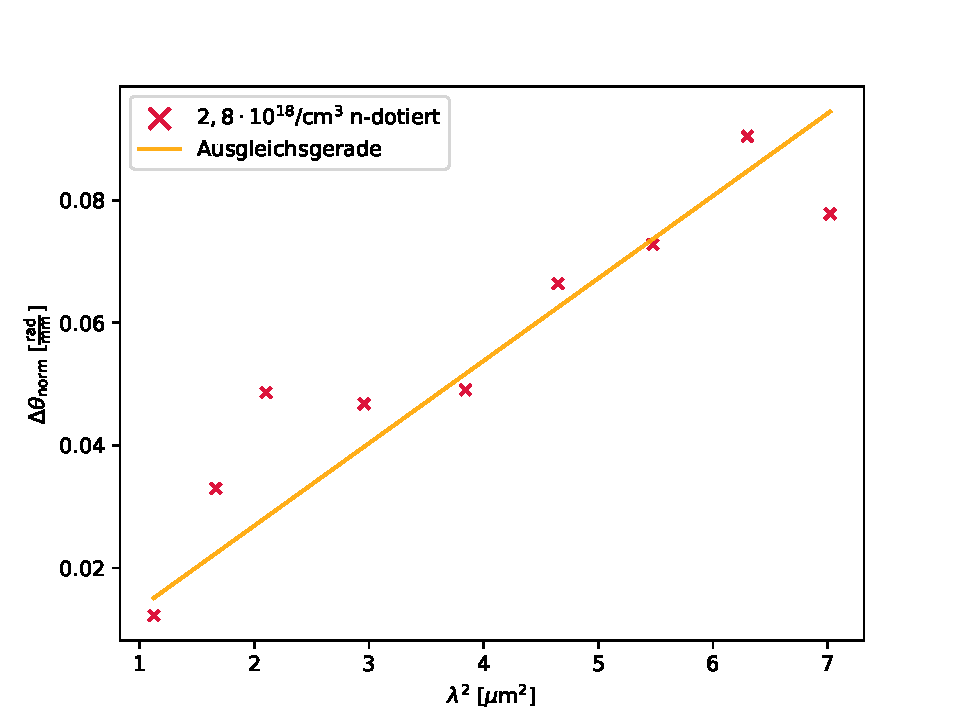
\includegraphics[width = 0.8\textwidth]{plots/Faraday_2.pdf}
            \caption{Die Differenz der Faraday-Rotation zwischen der hochreinen und zweiten dotierten Probe wird gegen die quadrierte Wellenlängeaufgetragen.}
            \label{fig:Faraday_2}
        \end{figure}

        \FloatBarrier

        Aus \eqref{eqn:faraday} kann also mithilfe der Steigung $a$ die effektive Masse bestimmt werden,
        \begin{equation*}
            m^* = \sqrt{\frac{\text{e}^3}{8\pi^2\varepsilon_0 \text{c}^3} \cdot \frac{N B_{\text{max}}}{n} \cdot \frac{1}{a}}
        \end{equation*}
        wobei der Brechungsindex $n \approx 3,34$ entnommen aus \cite{dargys_handbook_1994} ist, im Bereich der mittleren betrachteten Wellenlänge $\lambda_{\text{mittl}} \approx 1,904 \, \mu$m.

        Es ergeben sich jeweils für die beiden Proben die effektiven Massen von:
        \begin{align*}
            m^*_1 = (6,634 \pm 0,253) \cdot 10^{-32} \, \text{kg} \\[5pt]
            m^*_2 = (4,788 \pm 0,145) \cdot 10^{-32} \, \text{kg}
        \end{align*}
        In Anteilen von Elektronenmassen ist dies:
        \begin{align*}
            r_1 = \frac{m^*_1}{m_{\text{e}}} = (0,073 \pm 0,003) \\[7pt]
            r_2 = \frac{m^*_2}{m_{\text{e}}} = (0,053 \pm 0,002)
        \end{align*}

        Die relative Messabweichung vom Theoriewert für GaAs $r_{\text{th}} = \nicefrac{m^*}{m_{\text{e}}} \approx 0,067$ entnommen aus \cite{theeten_new_1978} ist jeweils:
        \begin{align*}
            A_1 &= \left|\frac{r_1 - r_{\text{th}}}{r_{\text{th}}}\right| \approx (8,70 \pm 4,15) \% \\[7pt]
            A_2 &= \left|\frac{r_2 - r_{\text{th}}}{r_{\text{th}}}\right| \approx (21,6 \pm 2,4) \%
        \end{align*}


















































